% Sections/05-ThietKeHeThong.tex
% Chương 5 -- Thiết kế hệ thống
%=========================

\section{Thiết kế hệ thống}
\label{sec:system-design}

Chương này chuyển các yêu cầu và quy trình đã phân tích ở chương trước thành thiết kế kỹ thuật cho hệ thống thương mại điện tử tích hợp AI Shopping Assistant. Nội dung tập trung vào cấu trúc thành phần, dữ liệu, giao tiếp, bảo mật và triển khai. Spring Boot Backend là cổng giao tiếp duy nhất của Frontend, còn MySQL là nguồn dữ liệu nghiệp vụ chính. AI Service hỗ trợ truy hồi và tư vấn nhưng không thay thế Backend trong việc xác nhận sản phẩm, giá, tồn kho và đơn hàng.

\subsection{Tổng quan và nguyên tắc thiết kế}

% \subsubsection{Phạm vi, mục tiêu và nguyên tắc thiết kế}

Hệ thống phục vụ hai nhóm tác nhân là khách hàng và quản trị viên. Khách hàng duyệt sản phẩm, tìm kiếm, sử dụng trợ lý hội thoại, quản lý giỏ hàng và đặt hàng; quản trị viên vận hành catalog, tồn kho, đơn hàng và đồng bộ chỉ mục AI. Phạm vi hiện tại sử dụng thanh toán khi nhận hàng (COD), chưa triển khai các cổng thanh toán trực tuyến. Ranh giới hệ thống gồm Frontend, Spring Boot Backend, AI Service và các kho dữ liệu do ứng dụng quản lý; các nhà cung cấp mô hình, lưu trữ ảnh và hạ tầng được truy cập qua adapter, không được client gọi trực tiếp.

Thiết kế hệ thống hướng đến các mục tiêu sau:

\begin{enumerate}[label=\arabic*., leftmargin=1.15cm]
    \item Tách nghiệp vụ thương mại điện tử khỏi AI và kiểm soát một cổng giao tiếp duy nhất từ Frontend đến Spring Boot Backend.
    \item Xem MySQL là nguồn dữ liệu chuẩn; Qdrant và kho checkpoint là các thành phần dẫn xuất có thể tái tạo hoặc thay thế.
    \item Hỗ trợ tìm kiếm văn bản, hình ảnh, kết hợp và hội thoại nhiều lượt thông qua các mô-đun AI có thể cấu hình.
    \item Đóng gói mô hình và dịch vụ bên ngoài sau adapter, đồng thời cô lập lỗi AI khỏi giỏ hàng, đặt hàng và tồn kho.
\end{enumerate}

Theo đó, Backend phải đối chiếu mọi mã sản phẩm do AI trả về với MySQL; các tích hợp bên ngoài phải có timeout, kiểm tra lỗi và phương án suy giảm phù hợp.

% \subsubsection{Các quyết định thiết kế tổng quát}

% Các quyết định thiết kế tổng quát được xây dựng từ nhóm yêu cầu phi chức năng ở chương phân tích. Bảng~\ref{tab:overview-architecture-decisions} tóm tắt cách các yêu cầu này được chuyển thành nguyên tắc tổ chức hệ thống.

% \begin{table}[H]
% \centering
% \footnotesize
% \caption{Ánh xạ yêu cầu phi chức năng với quyết định thiết kế}
% \label{tab:overview-architecture-decisions}
% \renewcommand{\arraystretch}{1.5}
% \setlength{\tabcolsep}{3.5pt}
% \begin{tabularx}{\linewidth}{|p{0.15\linewidth}|p{0.23\linewidth}|X|}
% \hline
% \textbf{Yêu cầu} & \textbf{Thuộc tính} & \textbf{Quyết định thiết kế} \\ \hline
% NFR-01 & Hiệu năng & Giới hạn số kết quả và tách các bước phân tích, embedding, retrieval, rerank để có thể đo thời gian từng bước. \\ \hline
% NFR-02 & Bảo mật & Sử dụng JWT, phân quyền theo vai trò, khóa API nội bộ và giới hạn truy cập MySQL, Qdrant trong mạng dịch vụ. \\ \hline
% NFR-03, NFR-04 & Khả dụng và tin cậy & Tách AI Service khỏi nghiệp vụ cốt lõi; MySQL giữ dữ liệu giao dịch và lỗi AI không làm mất hoặc sửa sai đơn hàng. \\ \hline
% NFR-05 & Bảo trì, mở rộng & Module hóa Frontend, Backend và AI Service; dùng adapter và biến môi trường để thay provider hoặc mô hình. \\ \hline
% NFR-06 & Tương thích & Frontend đáp ứng nhiều kích thước màn hình; các dịch vụ trao đổi dữ liệu JSON qua HTTP. \\ \hline
% NFR-07 & Khả năng quan sát & Cung cấp health check, metrics và log theo mã tương quan nhưng không ghi dữ liệu nhạy cảm. \\ \hline
% NFR-08 & Nhất quán & MySQL là nguồn chuẩn; Qdrant là chỉ mục có thể tái tạo; checkpoint hội thoại không thay thế dữ liệu giao dịch. \\ \hline
% NFR-09 & Tài nguyên AI & Cho phép bật, tắt hoặc thay thế embedding, reranker và phát hiện vật thể qua cấu hình. \\ \hline
% \end{tabularx}
% \end{table}

% Các nguyên tắc trên tạo thành tiêu chí kiểm soát cho những quyết định ở cấp mô-đun. Vì vậy, một thay đổi ở công nghệ AI hoặc dịch vụ tích hợp chỉ nên ảnh hưởng đến adapter và cấu hình liên quan; thay đổi đó không được làm thay đổi nguồn dữ liệu giao dịch, hợp đồng API công khai hoặc quy tắc xác nhận đơn hàng.

\subsection{Thiết kế kiến trúc hệ thống}

\subsubsection{Kiến trúc tổng thể}

Hệ thống gồm ba nhóm thành phần chính: lớp giao diện người dùng, lớp dịch vụ nội bộ và các dịch vụ, kho dữ liệu bên ngoài. Lớp giao diện sử dụng React và được phục vụ thông qua nginx. Lớp dịch vụ nội bộ gồm Spring Boot Backend và AI Service FastAPI. MySQL lưu dữ liệu nghiệp vụ, Qdrant lưu chỉ mục vector, còn các dịch vụ lưu trữ ảnh và nhà cung cấp mô hình hỗ trợ những chức năng bên ngoài hệ thống.

\begin{figure}[H]
    \centering
    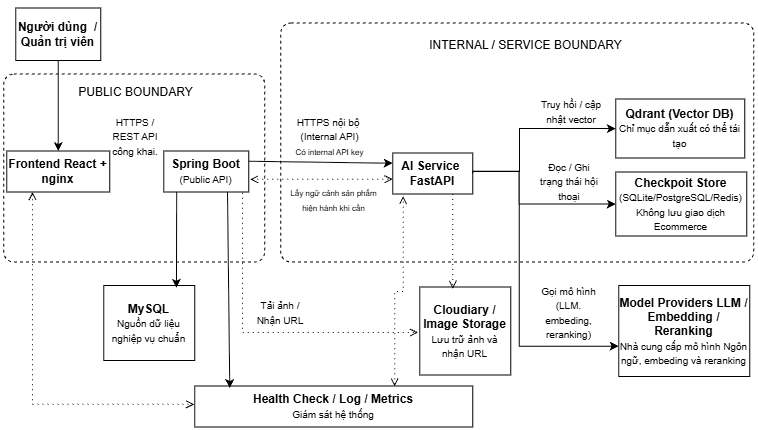
\includegraphics[width=0.98\textwidth]{Images/Thietkehethong/Kiến trúc tổng thể của hệ thống.drawio.drawio.png}
    \caption{Kiến trúc tổng thể của hệ thống}
    \label{fig:system-architecture}
\end{figure}

Hình~\ref{fig:system-architecture} phân chia hệ thống thành vùng truy cập công khai, vùng dịch vụ nội bộ và nhóm tích hợp bên ngoài. Frontend chỉ gọi Spring Boot bằng REST API; Backend xác thực, điều phối nghiệp vụ, truy cập MySQL và kiểm tra dữ liệu trước khi trả về client. Khi cần tìm kiếm hoặc tư vấn, Backend gọi AI Service qua API nội bộ có xác thực; AI Service dùng Qdrant, checkpoint và mô hình AI nhưng không truy cập trực tiếp MySQL. Cách phân lớp này giúp kiểm soát tập trung, hạn chế lộ thông tin kết nối và giữ cho lỗi của AI không ảnh hưởng đến các chức năng giao dịch chính. Vì vậy dữ liệu giao dịch, dữ liệu dẫn xuất và dịch vụ AI được tách biệt rõ ràng, thuận lợi cho bảo mật và mở rộng.

\subsubsection{Kiến trúc các thành phần ứng dụng}

\textbf{Kiến trúc phía máy khách.}

Frontend sử dụng React theo mô hình ứng dụng trang đơn. React Router quản lý định tuyến, Redux quản lý trạng thái dùng chung và lớp API tập trung giao tiếp với Backend. Cách tổ chức này giúp tái sử dụng thành phần giao diện và duy trì trạng thái nhất quán giữa các màn hình. Frontend chỉ hiển thị dữ liệu, tiếp nhận thao tác và hỗ trợ kiểm tra giao diện; quyền truy cập, giá bán, tồn kho và trạng thái đơn hàng vẫn phải được Backend xác minh. Frontend không lưu khóa AI và không kết nối trực tiếp đến MySQL hoặc Qdrant.
\clearpage
\begin{breakabletable}
    \centering
    \small
    \setlength{\tabcolsep}{3pt}
    \renewcommand{\arraystretch}{0.96}
    \caption{Các nhóm thành phần chính của Frontend}
    \label{tab:frontend-components}
    \begin{tabularx}{0.96\textwidth}{|p{0.24\textwidth}|X|}
        \hline
        \textbf{Nhóm thành phần} & \textbf{Trách nhiệm} \\
        \hline
        Trang và bố cục & Ghép các màn hình theo từng chức năng như trang chủ, sản phẩm, giỏ hàng, đơn hàng và quản trị. \\
        \hline
        Thành phần giao diện & Đóng gói các phần tử có thể dùng lại, hiển thị dữ liệu và phát sinh sự kiện từ thao tác người dùng. \\
        \hline
        Định tuyến & Ánh xạ URL đến màn hình tương ứng, điều hướng giữa các trang và giới hạn hiển thị các tuyến cần đăng nhập. \\
        \hline
        Redux và lưu trữ cục bộ & Lưu trạng thái dùng chung như người dùng hiện tại, giỏ hàng và trạng thái giao diện; không thay thế dữ liệu chuẩn trong MySQL. \\
        \hline
        API và tiện ích & Chuẩn hóa request đến Backend, gắn access token, chuyển đổi dữ liệu và xử lý các mã lỗi trả về. \\
        \hline
    \end{tabularx}
\end{breakabletable}

\textbf{Kiến trúc Spring Boot Backend.}

Backend được tổ chức theo kiến trúc phân lớp gồm bảo mật, Controller, Service, Repository và các bộ điều hợp tích hợp. Cách phân lớp tách phần tiếp nhận request, xử lý nghiệp vụ, truy cập dữ liệu và kết nối dịch vụ bên ngoài.

\begin{figure}[H]
    \centering
    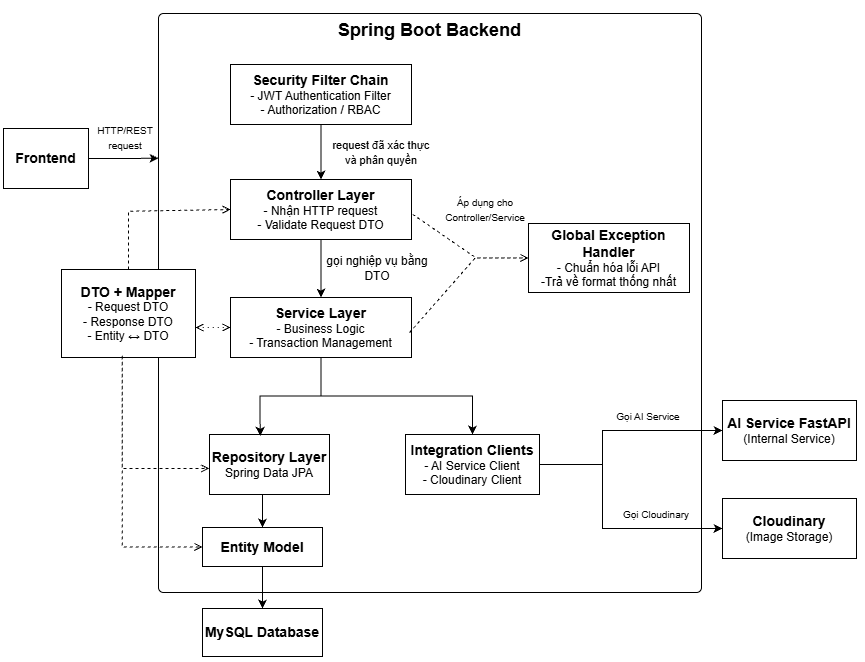
\includegraphics[width=0.91\textwidth]{Images/Thietkehethong/Kiến trúc phân lớp của Spring Boot Backend.drawio.png}
    \caption{Kiến trúc phân lớp của Spring Boot Backend}
    \label{fig:backend-layers}
\end{figure}

Như thể hiện ở Hình~\ref{fig:backend-layers}, JWT Authentication Filter xác thực request trước khi Controller tiếp nhận và kiểm tra dữ liệu. Controller chỉ điều phối, còn Service thực hiện các quy tắc như kiểm tra sản phẩm, tính giá, giữ tồn kho và tạo đơn hàng. Repository dùng Spring Data JPA để làm việc với MySQL; DTO bảo vệ ranh giới API và transaction bảo đảm các cập nhật liên quan thành công hoặc thất bại cùng nhau. Các adapter tập trung cấu hình địa chỉ, khóa, timeout và xử lý lỗi của dịch vụ bên ngoài.

\textbf{Kiến trúc AI Service.}

AI Service được xây dựng bằng FastAPI với ba tầng: API và schema, dịch vụ xử lý truy vấn/hội thoại/đồng bộ, cùng hạ tầng kết nối Qdrant, Backend, checkpoint và nhà cung cấp mô hình. Dịch vụ chuẩn hóa request, tạo vector, truy hồi và trả về Backend các mã sản phẩm, điểm phù hợp, nguồn kết quả và cảnh báo. AI Service không truy cập trực tiếp MySQL; Qdrant chỉ là chỉ mục dẫn xuất và khi một thành phần lỗi, dịch vụ trả kết quả suy giảm thay vì tạo dữ liệu giao dịch. Trách nhiệm từng mô-đun được tóm tắt tại Bảng~\ref{tab:ai-service-components}.

\begin{breakabletable}
    \centering
    \caption{Trách nhiệm các mô-đun chính của AI Service}
    \label{tab:ai-service-components}
    \begin{tabularx}{\textwidth}{|p{0.25\textwidth}|X|}
        \hline
        \textbf{Mô-đun} & \textbf{Trách nhiệm} \\
        \hline
        API và schema & Công bố endpoint, kiểm tra request và chuẩn hóa response. \\
        \hline
        Search và embedding & Phân tích truy vấn, xử lý văn bản/hình ảnh, tạo vector và truy vấn Qdrant. \\
        \hline
        Assistant và indexing & Phân loại yêu cầu, gọi công cụ, tạo câu trả lời, lưu trạng thái và cập nhật chỉ mục. \\
        \hline
        Infrastructure adapters & Đóng gói kết nối đến Qdrant, Backend, kho checkpoint và nhà cung cấp mô hình. \\
        \hline
    \end{tabularx}
\end{breakabletable}

% \subsubsection{Giao tiếp và phân chia trách nhiệm}

% Frontend chỉ gọi Backend bằng REST API; Backend xác thực người dùng, kiểm tra quyền và gọi AI Service qua mạng nội bộ bằng khóa dịch vụ, timeout và cấu trúc lỗi thống nhất. AI Service chỉ nhận dữ liệu cần thiết, không truy cập MySQL; mọi mã sản phẩm trả về đều được Backend đối chiếu lại với MySQL trước khi gửi cho Frontend. Khi AI lỗi, tìm kiếm văn bản có thể dùng fallback còn các nghiệp vụ cốt lõi vẫn hoạt động độc lập.

\subsection{Thiết kế dữ liệu và vòng đời dữ liệu}

Phần này trình bày cách tổ chức dữ liệu ở cấp hệ thống, quyền sở hữu của từng
kho lưu trữ và vòng đời của dữ liệu từ lúc phát sinh đến khi được sử dụng hoặc
tái tạo. Nội dung chính chỉ giữ các quyết định ảnh hưởng đến tính nhất quán,
khả năng truy vết và phối hợp giữa MySQL với các kho dữ liệu dẫn xuất. Từ điển
dữ liệu đầy đủ, gồm danh sách trường, kiểu dữ liệu và mô tả từng bảng, được
trình bày tại Phụ lục~\ref{appendix:data-dictionary} để tránh làm gián đoạn
luồng thiết kế trong chương này.

\subsubsection{Nguyên tắc và mô hình dữ liệu}

\textbf{Nguyên tắc tổ chức dữ liệu.}

Thiết kế dữ liệu tuân theo bốn nguyên tắc. Thứ nhất, dữ liệu giao dịch và dữ
liệu cần xác nhận cuối cùng phải thuộc quyền sở hữu của MySQL. Thứ hai, các
miền dữ liệu được phân tách theo trách nhiệm nghiệp vụ, nhưng vẫn liên kết qua
khóa định danh ổn định để hỗ trợ đối soát. Thứ ba, thông tin cần bảo toàn theo
thời điểm phát sinh, chẳng hạn giá, địa chỉ nhận hàng và dòng đơn hàng, được
chụp lại thay vì phụ thuộc hoàn toàn vào dữ liệu hiện hành. Thứ tư, dữ liệu
dẫn xuất như vector tìm kiếm, payload và checkpoint phải có nguồn gốc rõ ràng,
có thể cập nhật lại hoặc tái tạo khi cần.

\textbf{Quyền sở hữu và vòng đời dữ liệu.}

Bảng~\ref{tab:overview-data-ownership} phân định vai trò và quyền sở hữu của từng
kho, giúp hệ thống xử lý đúng khi dữ liệu dẫn xuất hoặc tạm thời chưa đồng bộ.

\begin{breakabletable}
\centering
\caption{Vai trò và quyền sở hữu dữ liệu của các kho lưu trữ}
\label{tab:overview-data-ownership}
\begin{tabularx}{\linewidth}{|p{0.20\linewidth}|p{0.28\linewidth}|X|}
\hline
\textbf{Kho dữ liệu} & \textbf{Vai trò} & \textbf{Nguyên tắc sử dụng} \\ \hline
MySQL & Lưu tài khoản, catalog, giá, tồn kho, giỏ hàng, đơn hàng và thanh toán. & Là nguồn dữ liệu nghiệp vụ chuẩn và được bảo vệ bằng giao dịch. \\ \hline
Qdrant & Lưu vector văn bản, vector hình ảnh và metadata truy hồi. & Là chỉ mục dẫn xuất; có thể tái tạo từ dữ liệu sản phẩm và không quyết định dữ liệu hiển thị cuối cùng. \\ \hline
Kho checkpoint & Lưu trạng thái workflow, tóm tắt, ràng buộc và lựa chọn theo phiên hội thoại. & Có thể dùng SQLite, PostgreSQL hoặc Redis theo môi trường; không lưu giao dịch thương mại điện tử. \\ \hline
Dịch vụ lưu trữ ảnh & Lưu tệp ảnh và cung cấp URL cho catalog hoặc truy vấn ảnh. & Backend kiểm tra tệp và chỉ lưu URL cần thiết trong dữ liệu sản phẩm. \\ \hline
Log và metrics & Lưu thông tin lỗi, latency và trạng thái vận hành. & Chỉ phục vụ quan sát, không chứa token, bí mật hoặc nội dung nhạy cảm không cần thiết. \\ \hline
\end{tabularx}
\end{breakabletable}

\textbf{Mô hình dữ liệu tổng quan.}

Dữ liệu MySQL được phân chia thành các miền nghiệp vụ nhằm giới hạn trách nhiệm
của từng nhóm bảng và thuận lợi cho việc bảo trì. Hình~\ref{fig:database-overview} thể hiện các
bảng, khóa chính, khóa ngoại quan trọng và quan hệ giữa các miền; thuộc tính chi
tiết của từng bảng được trình bày trong các sơ đồ thành phần ở phần tiếp theo.

\begin{figure}[H]
    \centering
    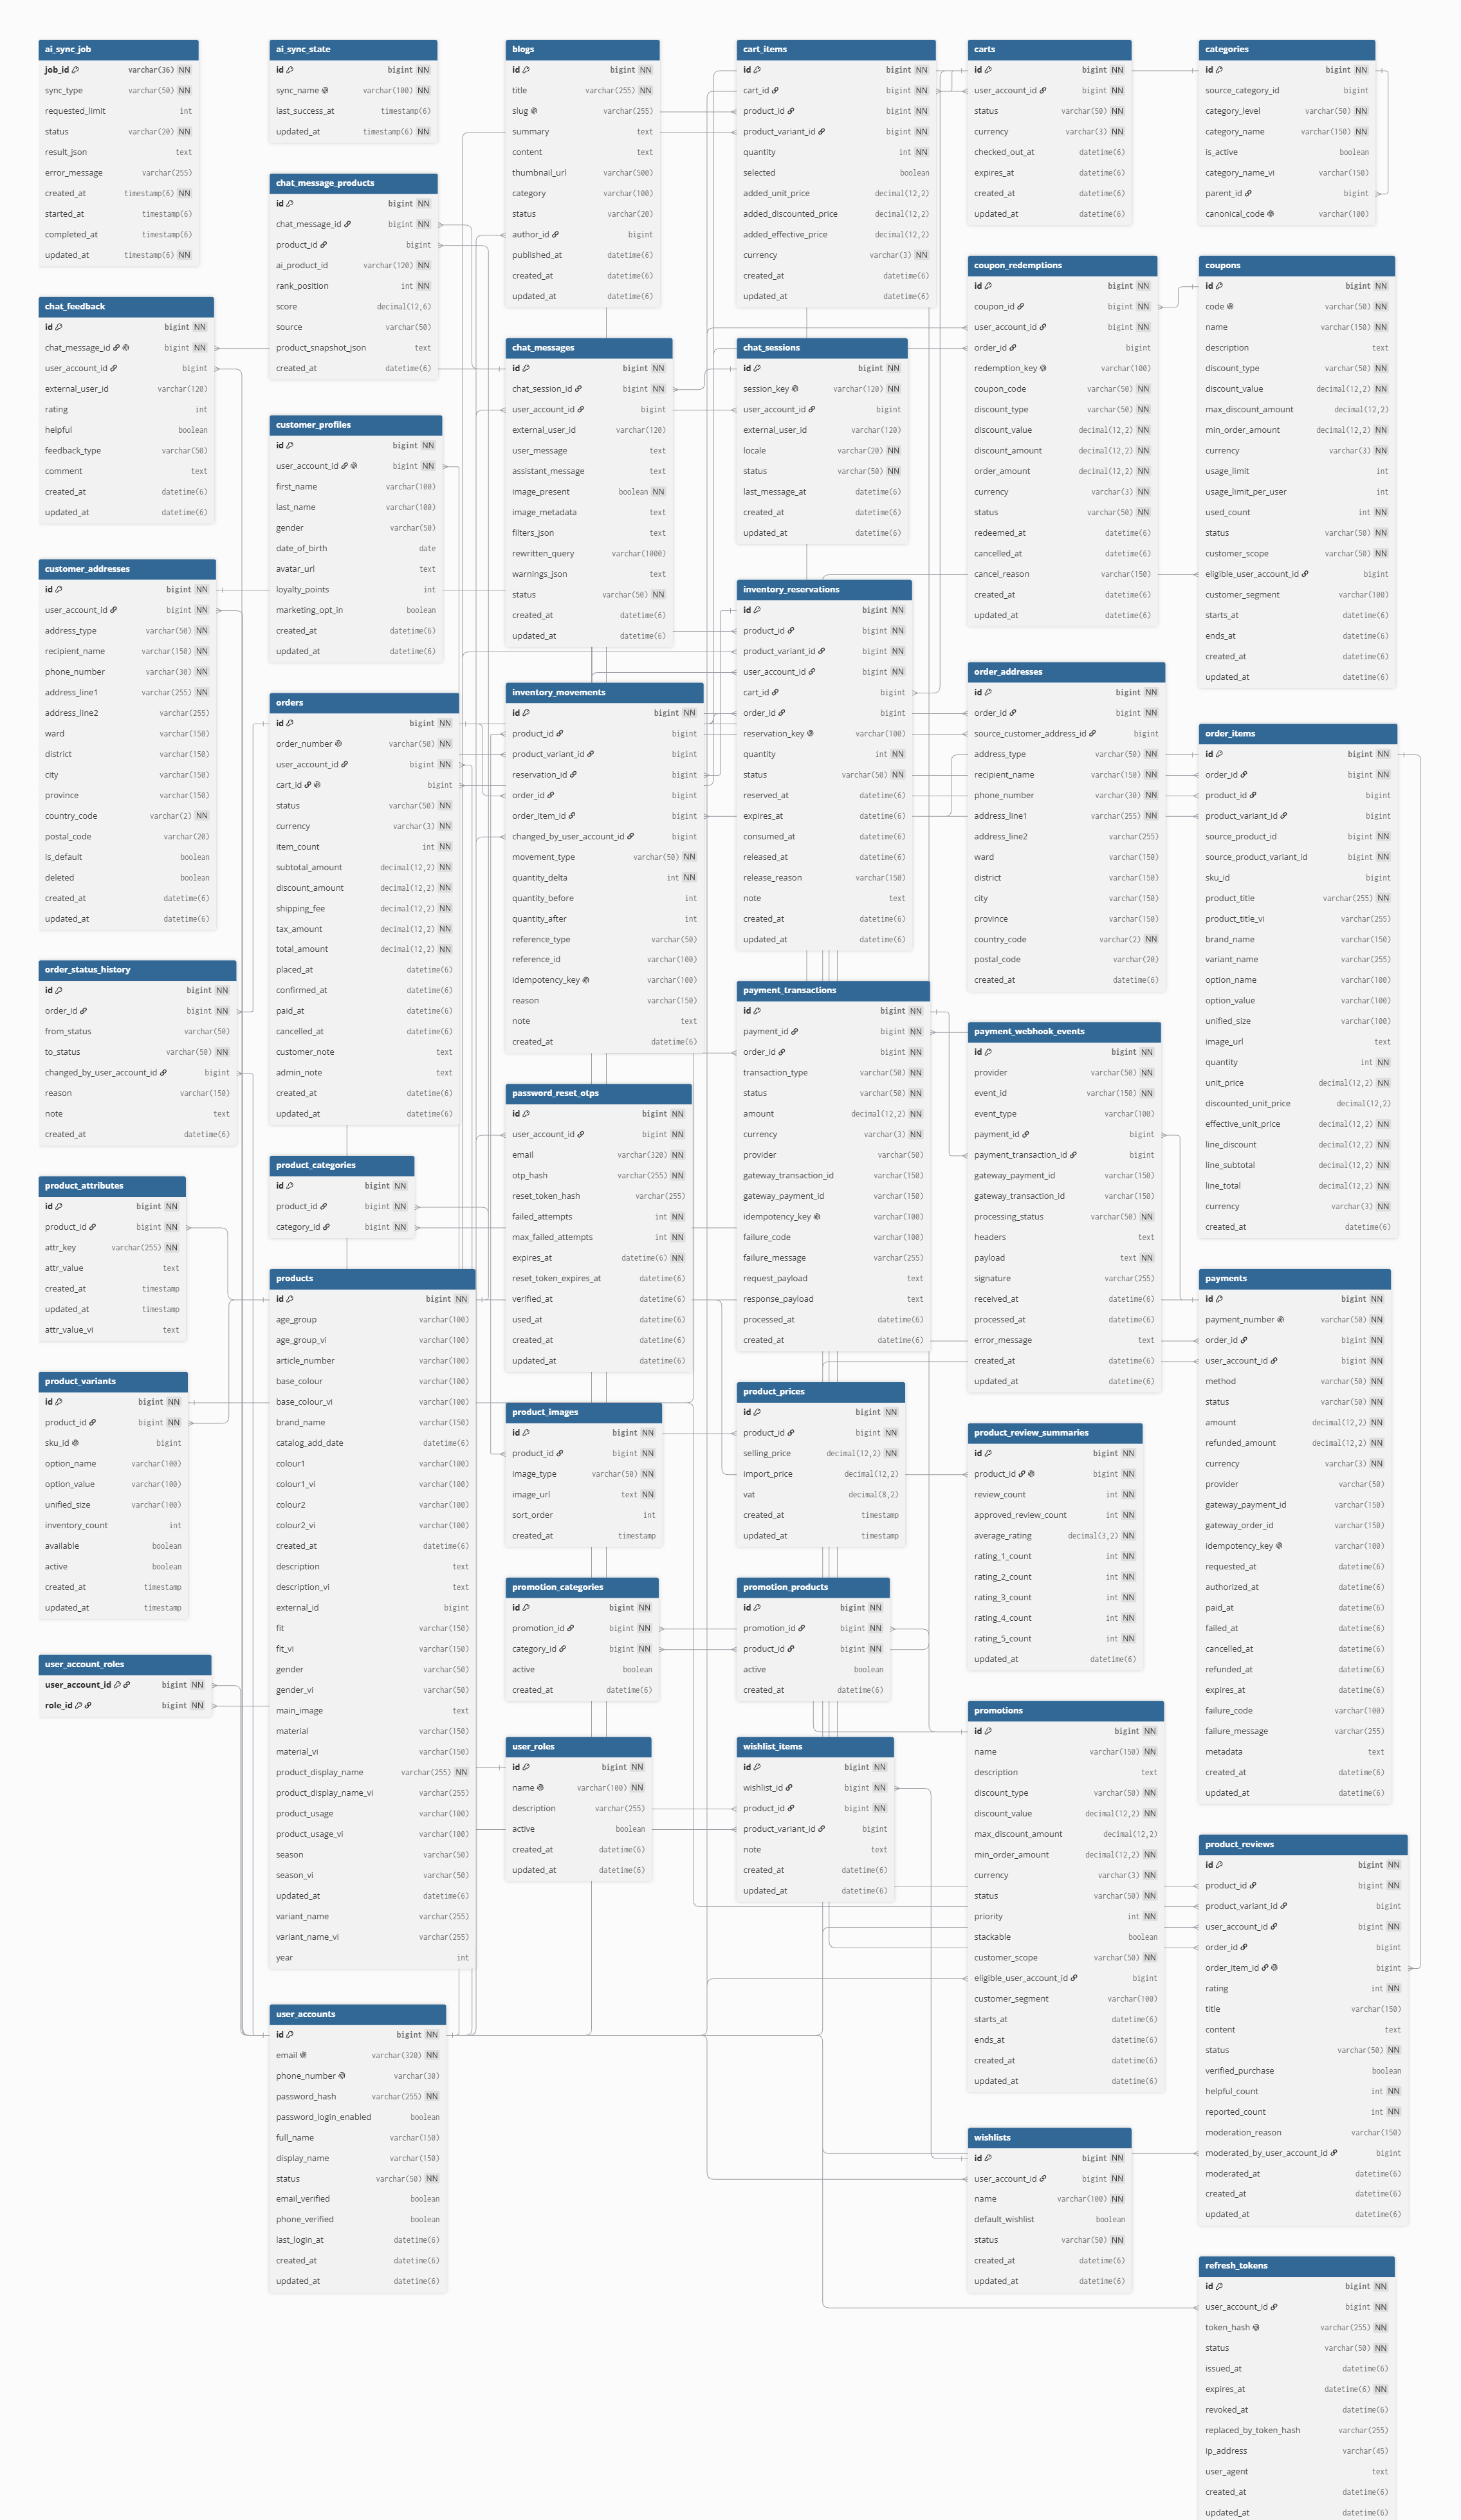
\includegraphics[
        width=\textwidth,
        height=1\textheight,
        keepaspectratio
    ]{Images/Thietkehethong/sơ đồ tổng quan toàn bộ cơ sở dữ liệu.png}
    \caption{Sơ đồ tổng quan toàn bộ cơ sở dữ liệu}
    \label{fig:database-overview}
\end{figure}

\subsubsection{Các miền dữ liệu nghiệp vụ}

\textbf{Nhóm dữ liệu người dùng và phân quyền.}

Nhóm này quản lý thông tin đăng nhập, hồ sơ, địa chỉ, vai trò và vòng đời thông
tin xác thực của người dùng. Quan hệ nhiều--nhiều giữa tài khoản và vai trò được
cài đặt qua bảng liên kết; refresh token và mã OTP khôi phục mật khẩu được lưu
riêng để có thể thu hồi, giới hạn thời gian sử dụng và truy vết độc lập.

\begin{figure}[H]
    \centering
    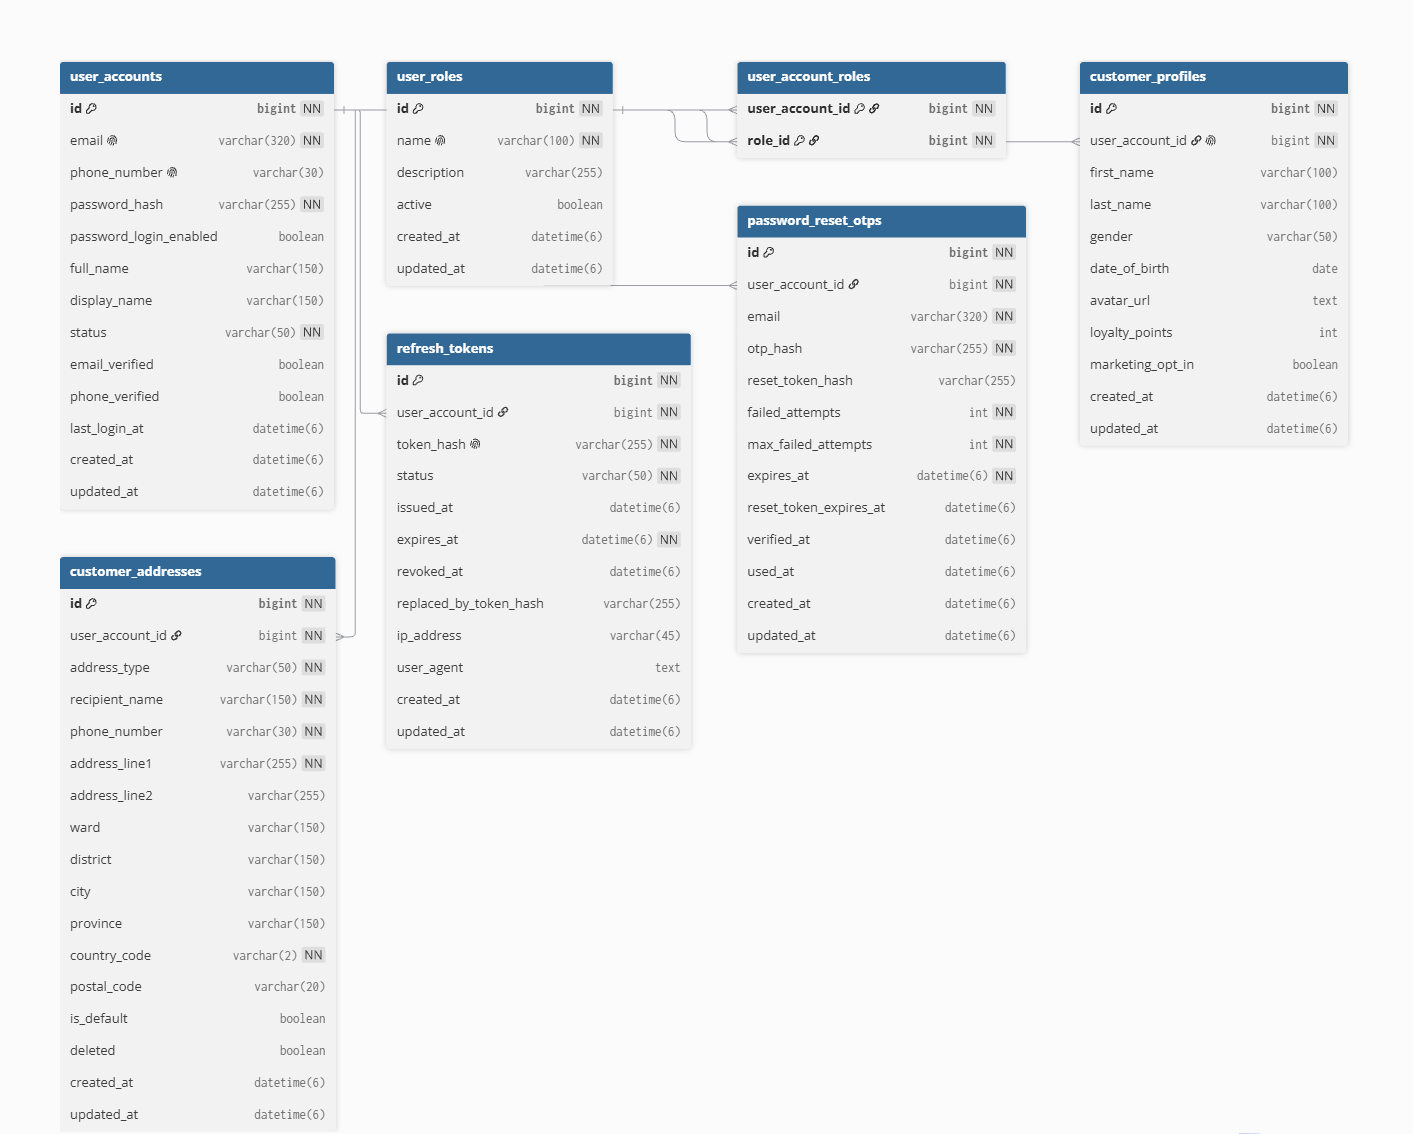
\includegraphics[
        width=\textwidth,
        height=0.72\textheight,
        keepaspectratio
    ]{Images/Thietkehethong/Người dùng và phân quyền.png}
    \caption{Sơ đồ dữ liệu người dùng và phân quyền}
    \label{fig:database-user-authorization}
\end{figure}

Trong Hình~\ref{fig:database-user-authorization}, \texttt{user\_accounts} là
thực thể trung tâm. Mỗi tài khoản có tối đa một hồ sơ khách hàng và có thể sở hữu
nhiều địa chỉ, refresh token hoặc yêu cầu đặt lại mật khẩu. Quan hệ giữa tài
khoản và vai trò được chuẩn hóa qua \texttt{user\_account\_roles}, cho phép mở
rộng tập vai trò mà không phải thay đổi cấu trúc tài khoản.

\textbf{Nhóm dữ liệu danh mục và sản phẩm.}

Nhóm danh mục và sản phẩm lưu dữ liệu mô tả hàng hóa, cấu trúc danh mục, biến
thể, thuộc tính, hình ảnh và giá bán. Bảng \texttt{products} đóng vai trò trung
tâm; các quan hệ thành phần được tách thành bảng riêng để một sản phẩm có thể có
nhiều danh mục, biến thể, thuộc tính và hình ảnh mà không lặp dữ liệu nền.

\begin{figure}[H]
    \centering
    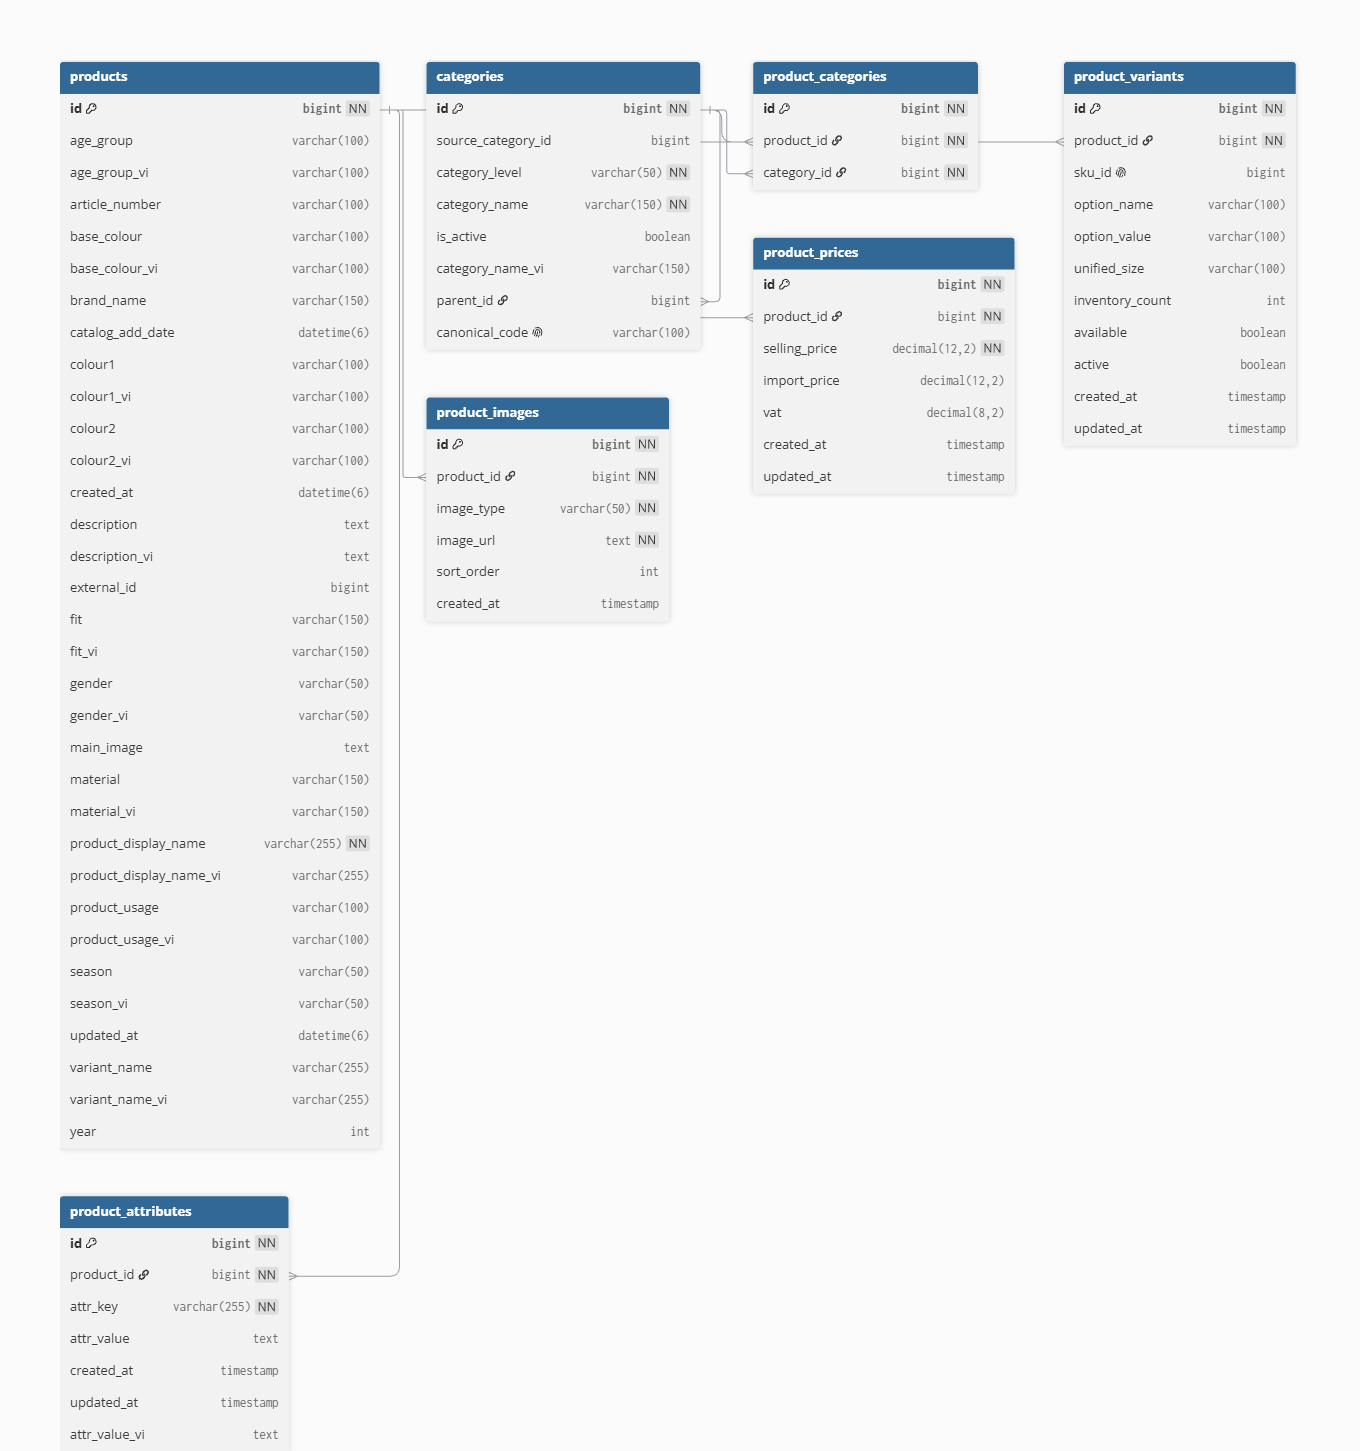
\includegraphics[
        width=\textwidth,
        height=0.72\textheight,
        keepaspectratio
    ]{Images/Thietkehethong/Danh mục và sản phẩm.png}
    \caption{Sơ đồ dữ liệu danh mục và sản phẩm}
    \label{fig:database-catalog-product}
\end{figure}

Hình~\ref{fig:database-catalog-product} cho thấy một sản phẩm có thể thuộc nhiều
danh mục thông qua bảng liên kết sản phẩm--danh mục; bản thân danh mục có quan hệ
cha--con để biểu diễn cấu trúc phân cấp. Biến thể, thuộc tính, hình ảnh và giá
được tách khỏi \texttt{products}, nhờ đó các tập dữ liệu có số lượng thay đổi
độc lập và không làm lặp lại thông tin mô tả chung của sản phẩm.

\textbf{Nhóm dữ liệu quản lý kho.}

Nhóm quản lý kho theo dõi phần hàng được giữ tạm trong quá trình đặt mua và lịch
sử thay đổi tồn kho. Mỗi bản ghi giữ hàng gắn với sản phẩm, biến thể, người dùng
và giỏ hoặc đơn hàng tương ứng; các biến động tồn kho lưu lượng thay đổi cùng
tham chiếu nghiệp vụ để hỗ trợ đối soát và chống xử lý trùng lặp.

\begin{figure}[H]
    \centering
    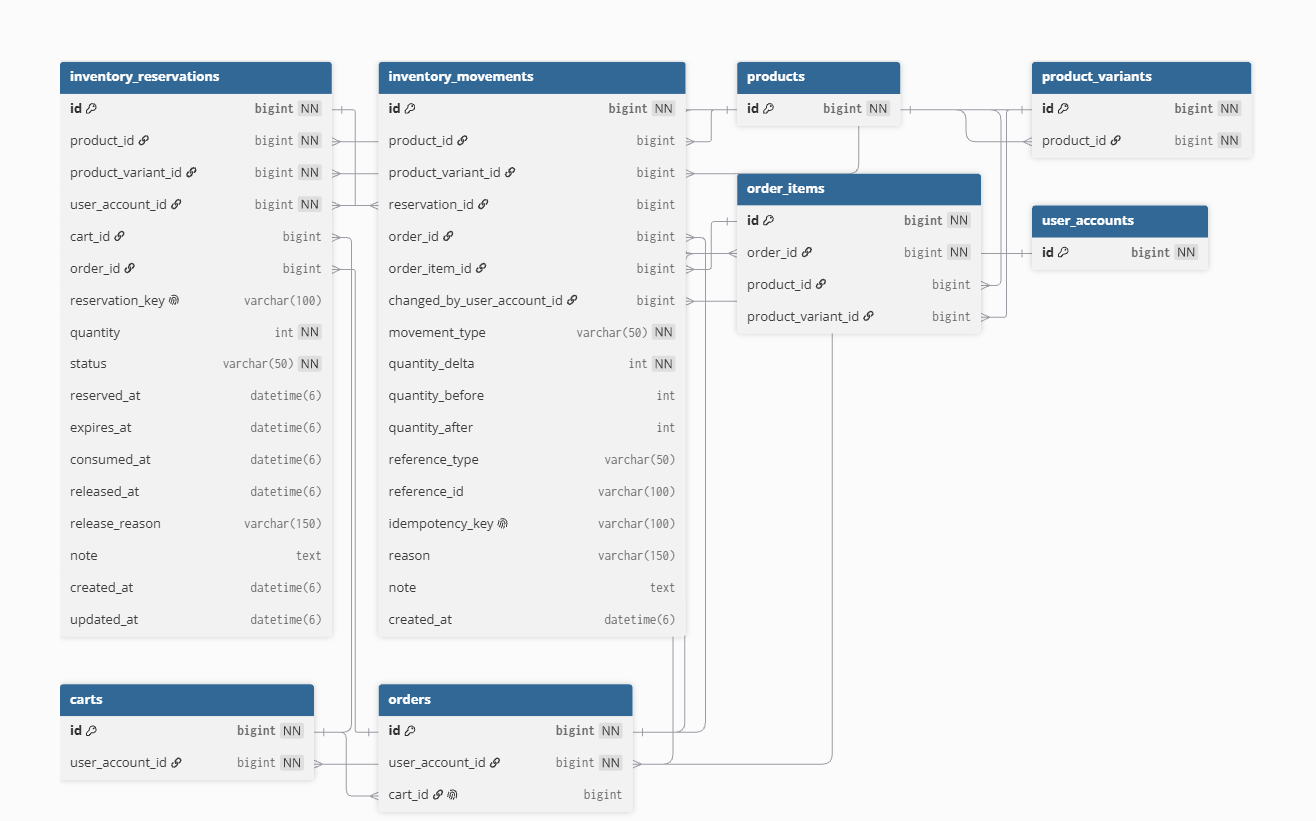
\includegraphics[
        width=\textwidth,
        height=0.72\textheight,
        keepaspectratio
    ]{Images/Thietkehethong/Quản lý kho.png}
    \caption{Sơ đồ dữ liệu quản lý kho}
    \label{fig:database-inventory}
\end{figure}

Theo Hình~\ref{fig:database-inventory},
\texttt{inventory\_reservations} biểu diễn phần tồn kho được giữ cho một người
dùng trong ngữ cảnh giỏ hàng hoặc đơn hàng. Mọi thay đổi tương ứng được ghi vào
\texttt{inventory\_movements} cùng lượng trước--sau, loại biến động và khóa
idempotency. Các bảng sản phẩm, giỏ hàng, đơn hàng và người dùng xuất hiện ở dạng
tham chiếu nhằm thể hiện nguồn phát sinh nghiệp vụ mà không lặp lại toàn bộ miền
dữ liệu liên quan.

\textbf{Nhóm dữ liệu giỏ hàng và tương tác khách hàng.}

Nhóm này lưu trạng thái giỏ hàng, các mặt hàng khách đã chọn, danh sách yêu thích,
đánh giá sản phẩm và nội dung blog phục vụ tương tác. Thông tin tổng hợp đánh giá
được tách khỏi đánh giá chi tiết để việc hiển thị số lượng và điểm trung bình
không phải tính lại trên toàn bộ dữ liệu sau mỗi truy vấn.

\begin{figure}[H]
    \centering
    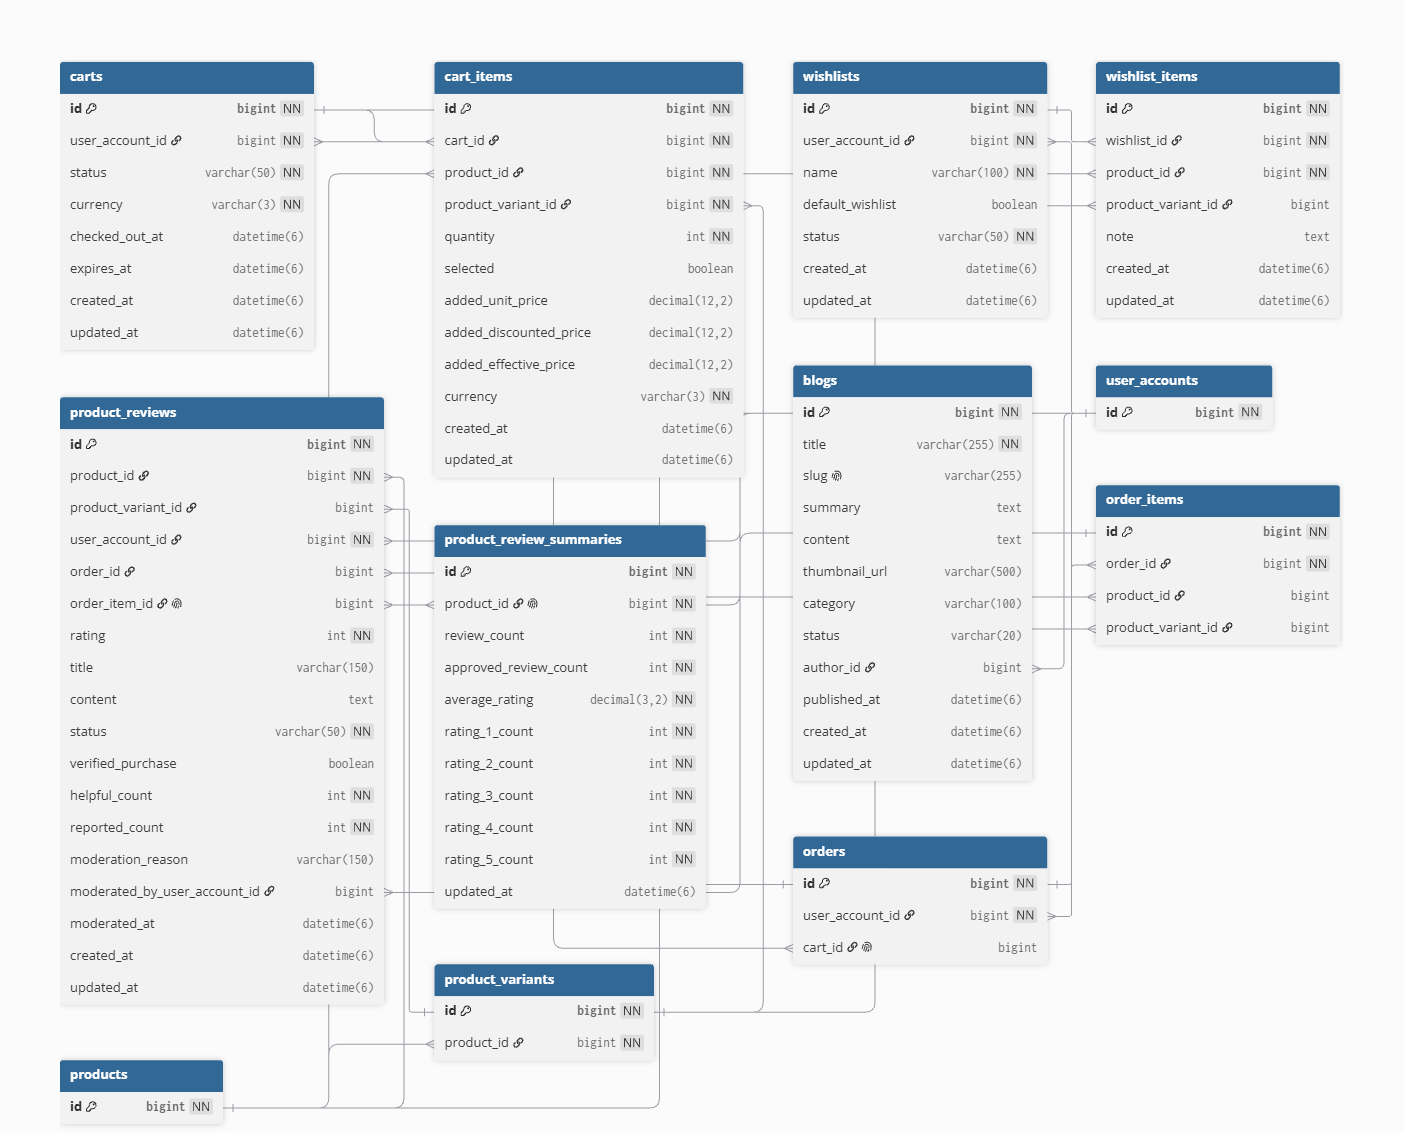
\includegraphics[
        width=\textwidth,
        height=0.72\textheight,
        keepaspectratio
    ]{Images/Thietkehethong/Giỏ hàng và tương tác khách hàng.png}
    \caption{Sơ đồ dữ liệu giỏ hàng và tương tác khách hàng}
    \label{fig:database-cart-engagement}
\end{figure}

Hình~\ref{fig:database-cart-engagement} tập hợp các dữ liệu phát sinh từ quá
trình tương tác của khách hàng. Giỏ hàng và danh sách yêu thích đều được tổ chức
theo mô hình bảng đầu mục--chi tiết. Đánh giá liên kết với người dùng, sản phẩm
và dòng đơn hàng để xác minh giao dịch mua, trong khi
\texttt{product\_review\_summaries} lưu kết quả tổng hợp phục vụ truy vấn đọc.
Bài viết blog liên kết tùy chọn với tài khoản tác giả và không phụ thuộc vào vòng
đời mua hàng.

\textbf{Nhóm dữ liệu đơn hàng và vận chuyển.}

Nhóm đơn hàng lưu kết quả của quá trình mua sắm, các dòng hàng, bản chụp địa chỉ
nhận hàng và lịch sử chuyển trạng thái. Giá, tên và thuộc tính cần thiết của sản
phẩm được chụp lại trong \texttt{order\_items}; do đó nội dung đơn đã phát sinh
không bị thay đổi khi dữ liệu sản phẩm hiện hành được cập nhật hoặc xóa.

\begin{figure}[H]
    \centering
    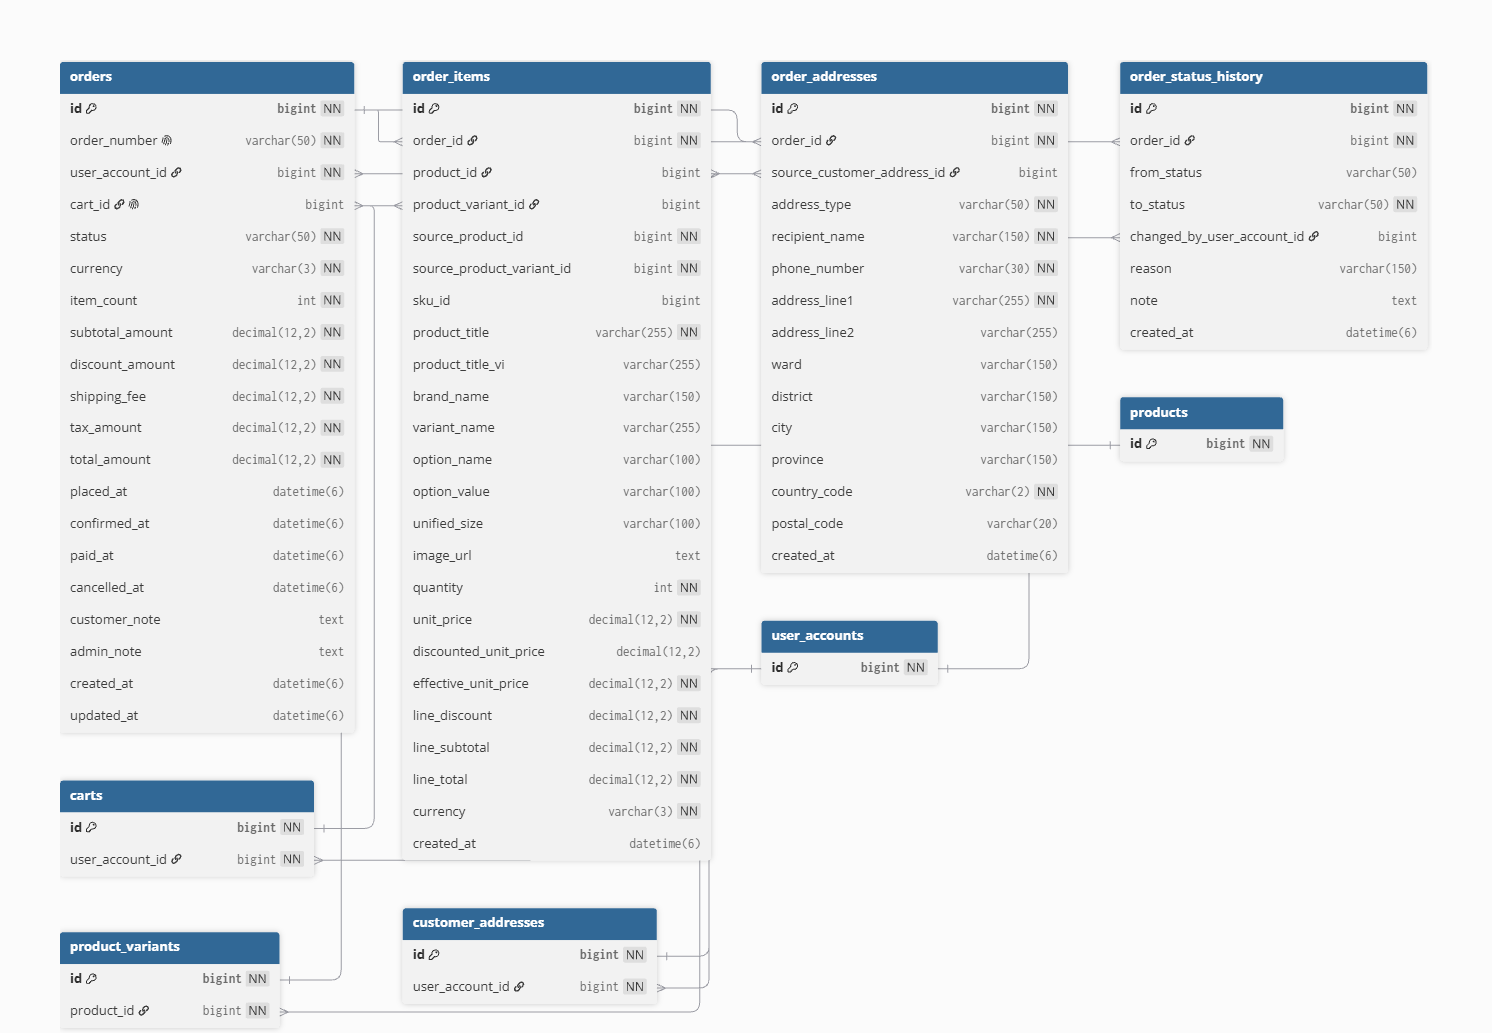
\includegraphics[
        width=\textwidth,
        height=0.72\textheight,
        keepaspectratio
    ]{Images/Thietkehethong/Đơn hàng và vận chuyển.png}
    \caption{Sơ đồ dữ liệu đơn hàng và vận chuyển}
    \label{fig:database-order-shipping}
\end{figure}

Trong Hình~\ref{fig:database-order-shipping}, \texttt{orders} liên kết một--nhiều
với các dòng hàng, địa chỉ chụp tại thời điểm đặt và lịch sử trạng thái. Liên kết
đến sản phẩm và biến thể được phép rỗng để đơn hàng cũ vẫn tồn tại khi dữ liệu
danh mục thay đổi. Tương tự, \texttt{order\_addresses} giữ bản sao địa chỉ giao
nhận thay vì phụ thuộc hoàn toàn vào địa chỉ hiện hành trong hồ sơ khách hàng.

\textbf{Nhóm dữ liệu thanh toán và khuyến mãi.}

Nhóm này quản lý khoản thanh toán của đơn hàng, từng giao dịch với nhà cung cấp,
sự kiện webhook và các chính sách giảm giá. Khuyến mãi có thể giới hạn theo sản
phẩm hoặc danh mục, trong khi lịch sử đổi coupon lưu bản chụp giá trị giảm và
trạng thái sử dụng để hỗ trợ kiểm tra, hủy hoặc hoàn tác đơn hàng.

\begin{figure}[H]
    \centering
    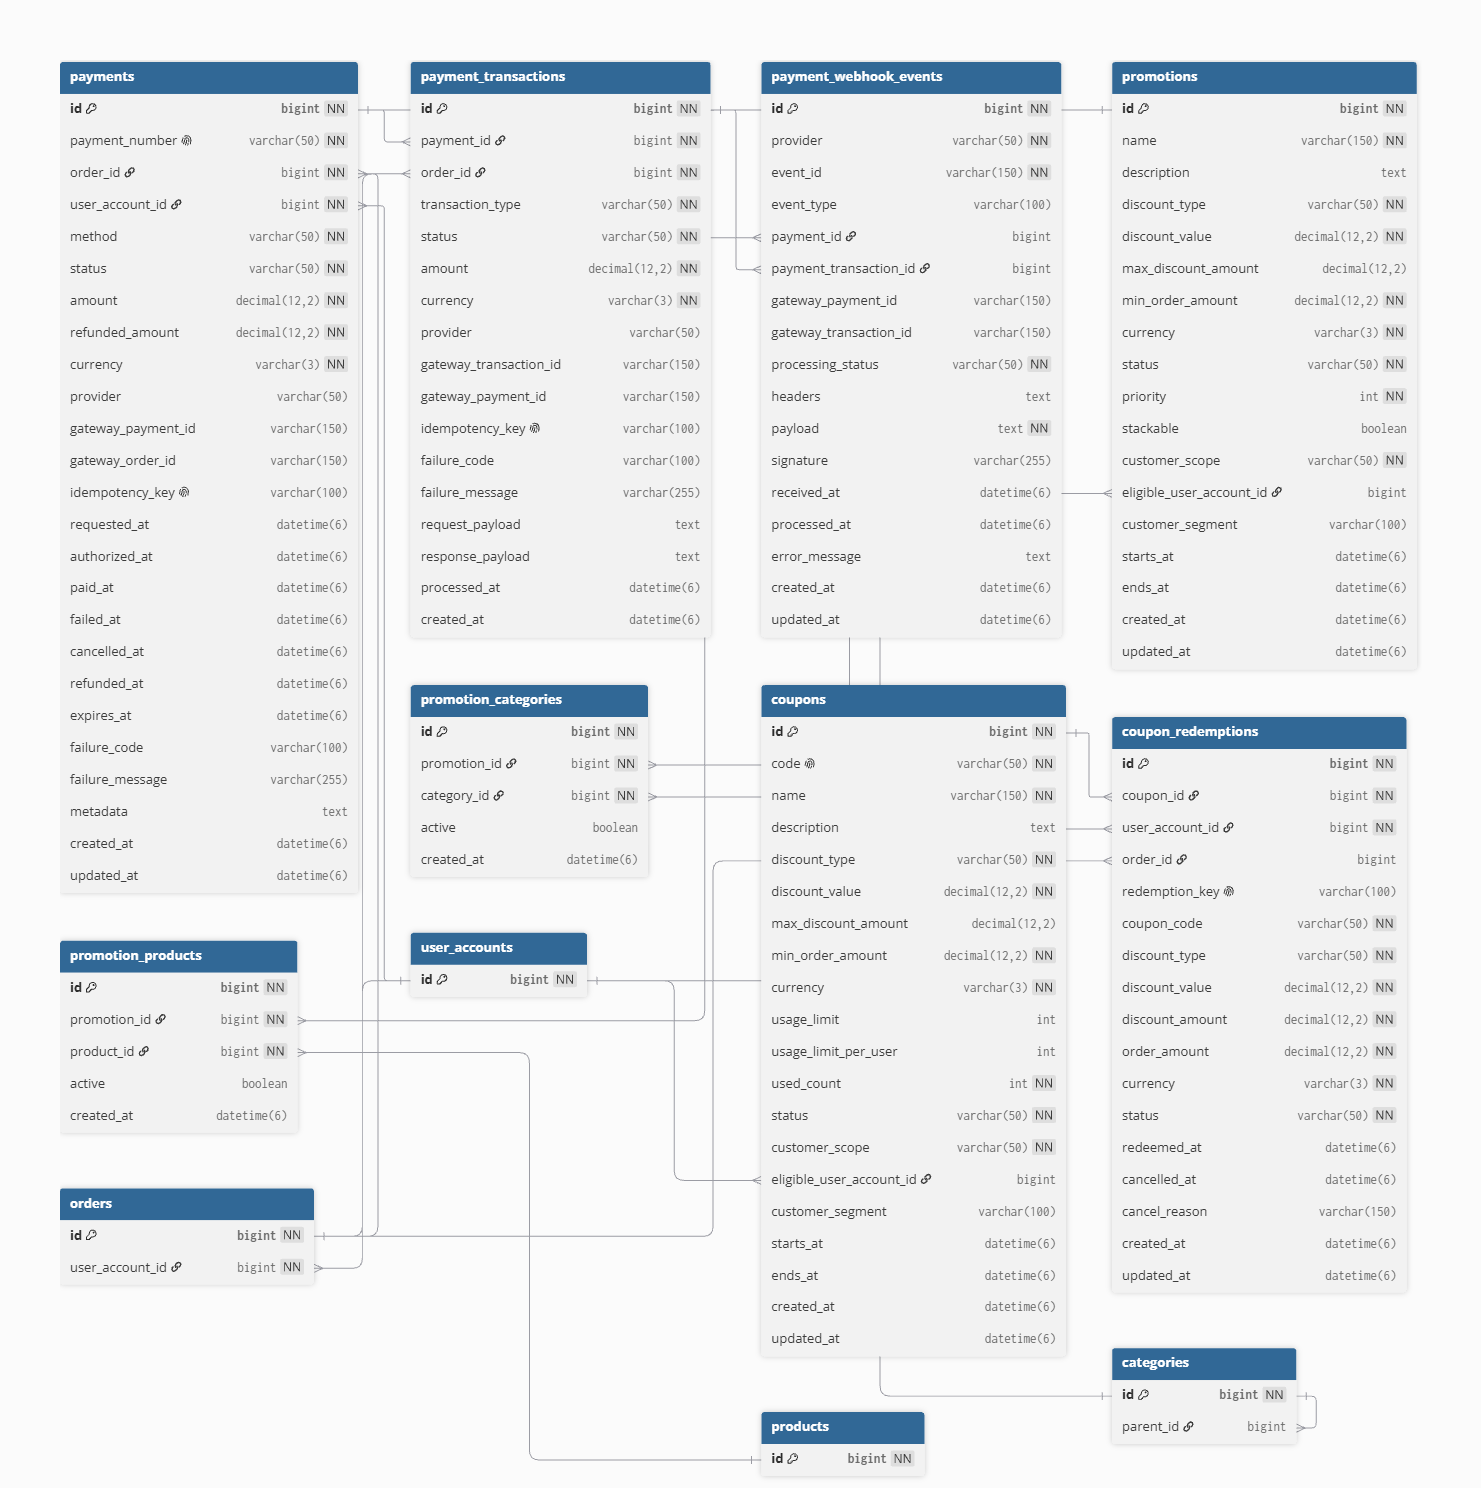
\includegraphics[
        width=\textwidth,
        height=0.72\textheight,
        keepaspectratio
    ]{Images/Thietkehethong/Thanh toán và khuyến mãi.png}
    \caption{Sơ đồ dữ liệu thanh toán và khuyến mãi}
    \label{fig:database-payment-promotion}
\end{figure}

Hình~\ref{fig:database-payment-promotion} thể hiện ba cụm quan hệ chính. Cụm
thanh toán liên kết \texttt{payments} với các lần giao dịch và sự kiện webhook
để hỗ trợ đối soát. Cụm khuyến mãi dùng các bảng liên kết để giới hạn phạm vi
theo sản phẩm hoặc danh mục. Cụm coupon ghi nhận lượt sử dụng theo người dùng và
đơn hàng, đồng thời chụp lại loại giảm, giá trị giảm và số tiền thực tế để bảo
toàn lịch sử tính giá.

\subsubsection{Dữ liệu AI và đồng bộ chỉ mục}

\textbf{Nhóm dữ liệu tích hợp và đồng bộ AI.}

Nhóm tích hợp AI lưu trạng thái các công việc đồng bộ, mốc đồng bộ thành công gần
nhất và dữ liệu hội thoại của trợ lý. Phiên, tin nhắn, sản phẩm được gợi ý và phản
hồi của người dùng được tách riêng để hỗ trợ hội thoại nhiều lượt, đánh giá chất
lượng kết quả và truy vết sản phẩm đã được AI sử dụng trong câu trả lời.

\begin{figure}[H]
    \centering
    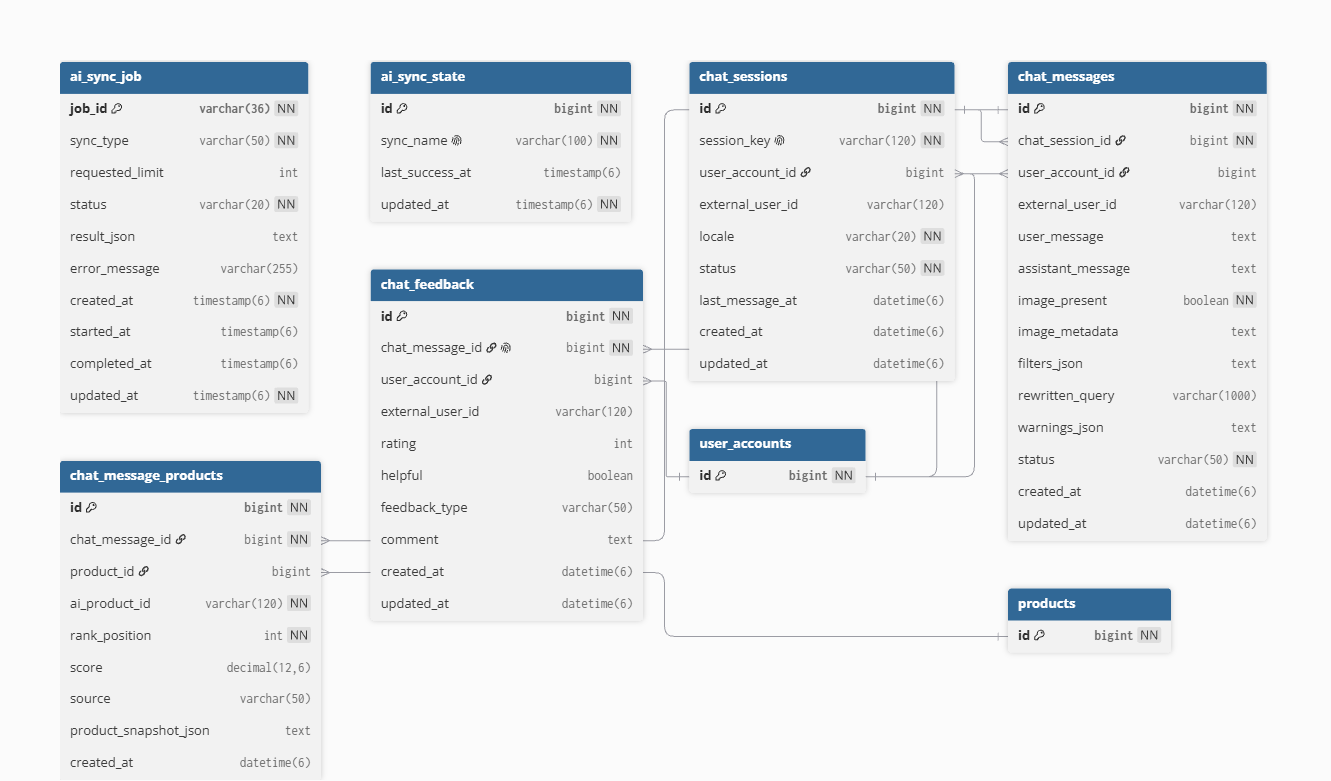
\includegraphics[
        width=\textwidth,
        height=0.72\textheight,
        keepaspectratio
    ]{Images/Thietkehethong/Tích hợp và đồng bộ AI.png}
    \caption{Sơ đồ dữ liệu tích hợp và đồng bộ AI}
    \label{fig:database-ai-integration}
\end{figure}

Theo Hình~\ref{fig:database-ai-integration}, một phiên hội thoại gồm nhiều tin
nhắn; mỗi tin nhắn có thể gắn với các sản phẩm được AI đề xuất và tối đa một phản
hồi đánh giá. Liên kết đến tài khoản và sản phẩm có thể rỗng để hỗ trợ khách chưa
đăng nhập cũng như bảo toàn bản chụp kết quả AI. Hai bảng
\texttt{ai\_sync\_job} và \texttt{ai\_sync\_state} không có khóa ngoại với
cụm hội thoại vì chúng theo dõi tiến trình lập chỉ mục ở cấp hệ thống, thay vì
biểu diễn một lượt tương tác của người dùng.

\textbf{Thiết kế chỉ mục và đồng bộ dữ liệu MySQL--Qdrant.}

MySQL là nguồn dữ liệu chuẩn, còn Qdrant chỉ lưu dữ liệu dẫn xuất phục vụ truy hồi. Mỗi điểm trong chỉ mục sử dụng \texttt{product\_id} làm khóa liên kết ổn định với sản phẩm trong MySQL. Vector văn bản và vector hình ảnh có thể được tổ chức trong các collection riêng do khác nhau về mô hình embedding, số chiều và chiến lược truy vấn. Payload chỉ chứa metadata cần thiết cho lọc và xếp hạng, chẳng hạn danh mục, thuộc tính, khoảng giá, trạng thái khả dụng và thời điểm cập nhật.

Giá, tồn kho và trạng thái trong payload là ảnh chụp nên Qdrant chỉ dùng để tìm ứng
viên; Spring Boot luôn nạp lại dữ liệu hiện hành từ MySQL trước khi trả kết quả.
Hệ thống hỗ trợ đồng bộ toàn bộ, tăng dần, theo sản phẩm và xóa; các thao tác dùng
\texttt{product\_id} ổn định nên có thể thực hiện lại an toàn theo luồng tại
Hình~\ref{fig:ai-sync-flow}.

\begin{figure}[H]
    \centering
    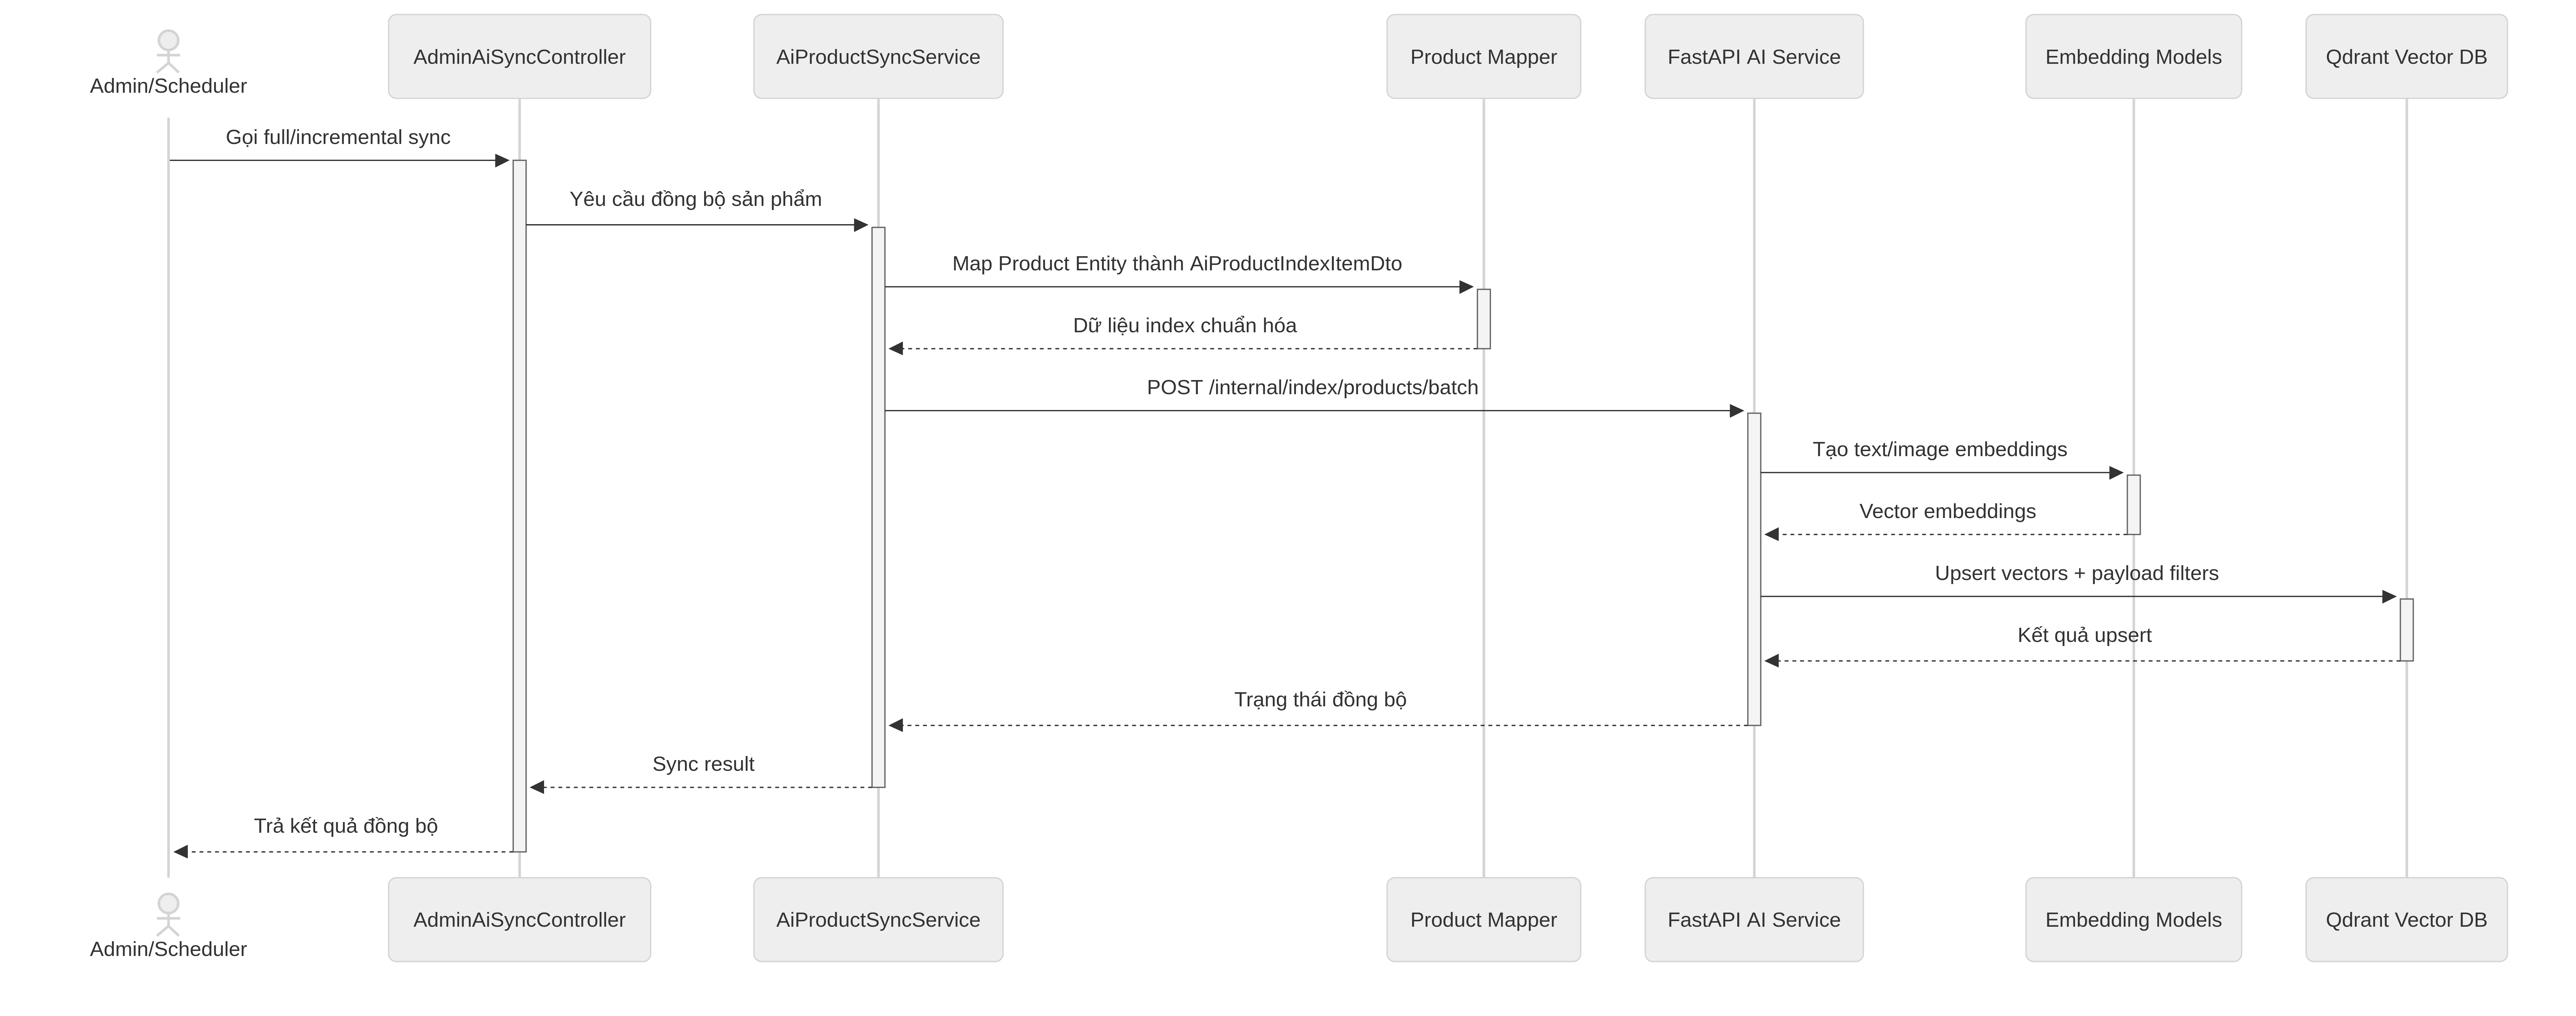
\includegraphics[
        width=0.95\textwidth
    ]{Images/Thietkehethong/dongboAI.png}
    \caption{Luồng đồng bộ dữ liệu từ MySQL sang Qdrant}
    \label{fig:ai-sync-flow}
\end{figure}

Tiến trình được ghi nhận trong \texttt{ai\_sync\_job} và \texttt{ai\_sync\_state};
thành công một phần hoặc lỗi đều ghi nhận bản ghi cần thử lại. Lỗi cập nhật Qdrant
không hoàn tác giao dịch MySQL vì chỉ mục có thể được tái tạo.

\subsection{Thiết kế các chức năng cốt lõi}

Các sơ đồ hoạt động chính đã được trình bày tại Chương~\ref{sec:requirements-analysis}. Phần này tập trung vào
các quyết định bên trong như kiểm tra dữ liệu, transaction, chuyển trạng thái và
cách xử lý khi dịch vụ phụ thuộc không khả dụng. Dữ liệu giao dịch được kiểm tra
và lưu tại Backend, còn kết quả AI chỉ được dùng như dữ liệu hỗ trợ có thể xác minh.

% \subsubsection{Luồng xử lý tổng quát}
\textbf{Luồng xử lý tổng quát.}

Luồng xử lý tổng quát gồm ba luồng chính : (i) luồng thương mại điện tử đi từ Frontend qua Spring Boot,
kiểm tra quyền và nghiệp vụ rồi đọc/ghi MySQL; (ii) luồng AI trực tuyến tiếp nhận
văn bản, ảnh hoặc hội thoại, truy hồi Qdrant và trả mã sản phẩm để Backend xác minh;
(iii) luồng đồng bộ chỉ mục đọc dữ liệu MySQL theo batch, tạo embedding và cập nhật
Qdrant. Lỗi đồng bộ chỉ mục được ghi nhận để thử lại, không hoàn tác giao dịch MySQL;
do đó các nghiệp vụ catalog, giỏ hàng và đặt hàng vẫn hoạt động khi AI suy giảm.

\subsubsection{Checkout và quản lý vòng đời đơn hàng}

Checkout tách thành hai bước. Preview chỉ tính giá, giảm giá và coupon dự kiến; confirm kiểm tra lại giỏ hàng, địa chỉ, sản phẩm, tồn kho và coupon trong transaction trước khi tạo đơn.

Khi hợp lệ, Backend tạo \texttt{Order}, lưu thông tin tại thời điểm đặt hàng, giữ tồn kho và ghi lịch sử trạng thái. Nếu một bước ghi bắt buộc thất bại, transaction được rollback. Luồng đặt hàng COD được thể hiện tại Hình~\ref{fig:activity-cod-checkout}; phần xác nhận được trình bày tại Hình~\ref{appendix:fig:activity-cod-confirmation} ở phụ lục.

Trạng thái đơn hàng được quản lý bằng các chuyển tiếp hợp lệ. Mỗi chuyển tiếp kiểm tra trạng thái hiện tại, vai trò người thực hiện và tác động đến tồn kho hoặc thanh toán; lịch sử được ghi lại để truy vết.

\begin{figure}[H]
    \centering
    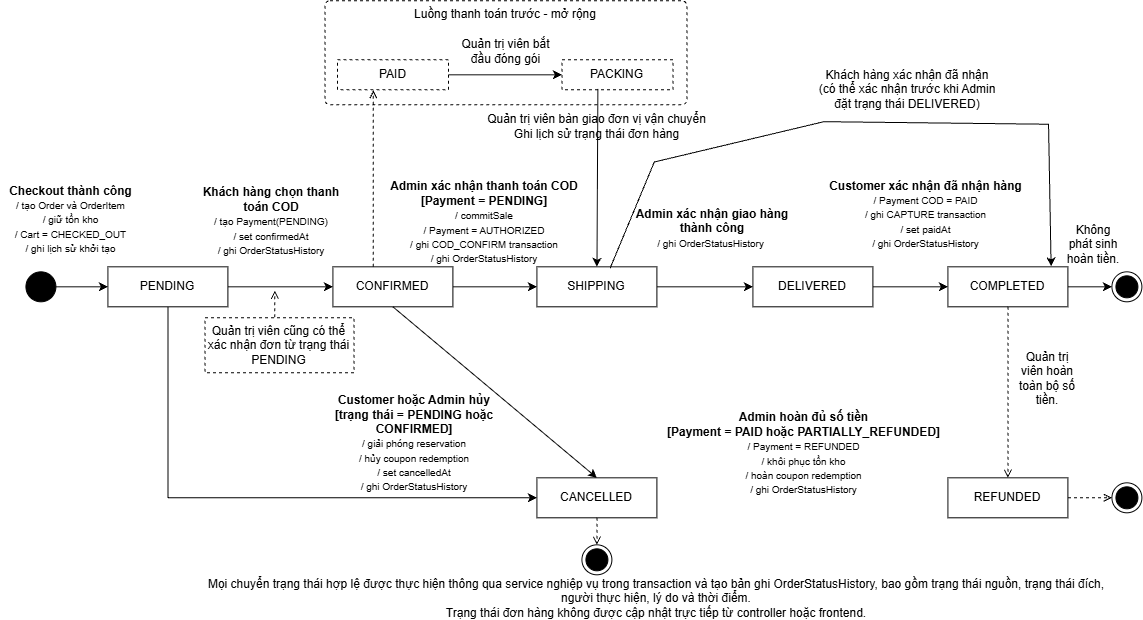
\includegraphics[width=0.98\textwidth]{Images/Thietkehethong/Thiết kế vòng đời trạng thái đơn hàng và các tác động nghiệp vụ.drawio.png}
    \caption{Thiết kế vòng đời trạng thái đơn hàng và các tác động nghiệp vụ}
    \label{fig:order-state-design}
\end{figure}

Hình~\ref{fig:order-state-design} mô tả vòng đời COD từ PENDING, CONFIRMED,
SHIPPING đến DELIVERED; mỗi chuyển tiếp kiểm tra trạng thái hiện tại, vai trò và tác
động đến tồn kho hoặc thanh toán. Đơn chỉ được hủy ở các trạng thái hợp lệ; thao tác
hủy hoặc hoàn tiền phải khôi phục tồn kho/coupon và ghi lịch sử. Nhánh thanh toán
trước chỉ là hướng mở rộng, còn mọi chuyển tiếp hiện tại đều đi qua service nghiệp
vụ trong transaction và không được cập nhật trực tiếp tại Controller.
\subsubsection{Các chức năng AI}

\textbf{Tìm kiếm sản phẩm bằng AI.}

Luồng tương tác đa phương thức đã được mô tả tại Hình~\ref{fig:activity-multimodal-search}. Request gồm văn bản, ảnh, vùng quan tâm, bộ lọc và giới hạn kết quả; endpoint \texttt{auto} chọn nhánh xử lý phù hợp. Pipeline gồm chuẩn hóa truy vấn, xử lý ảnh, tạo embedding và truy hồi Qdrant; reranking và YOLO là các bước tùy chọn.

\begin{figure}[H]
    \centering
    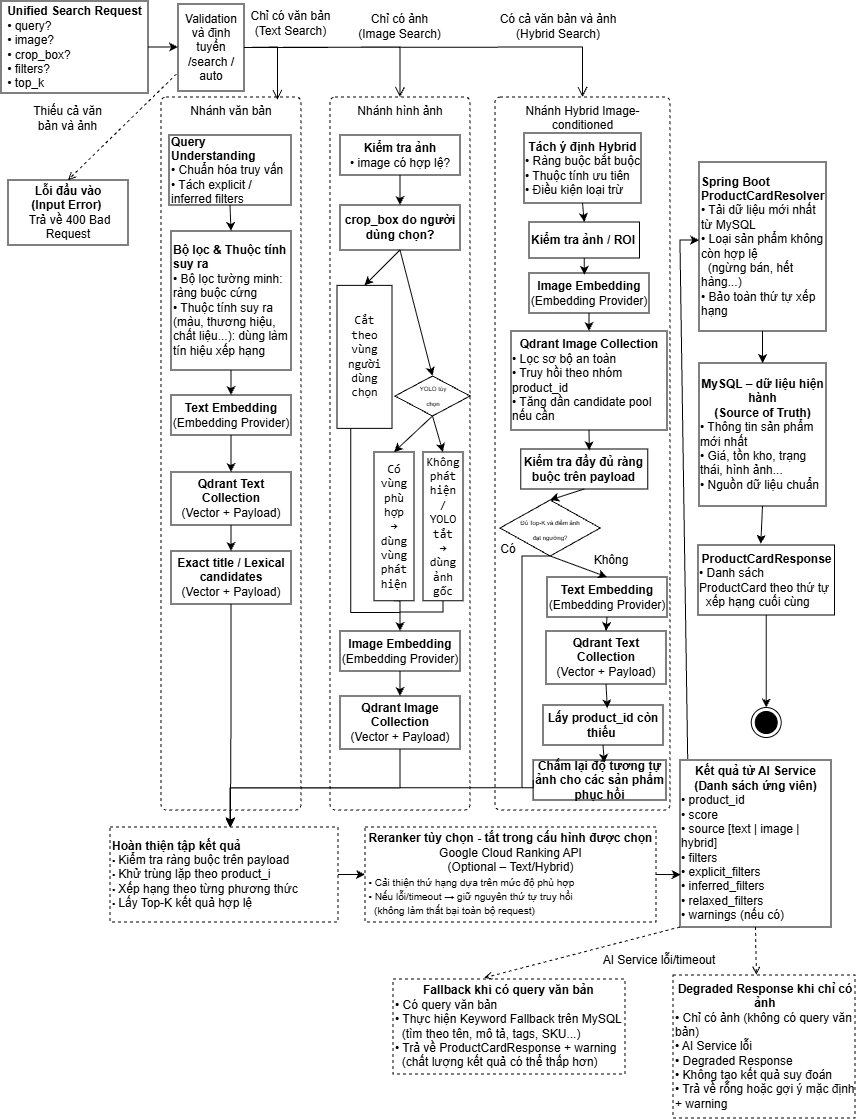
\includegraphics[width=0.92\textwidth,height=0.78\textheight,keepaspectratio]{Images/Thietkehethong/Pipeline xử lý tìm kiếm sản phẩm đa phương thức.drawio.png}
    \caption{Pipeline xử lý tìm kiếm sản phẩm đa phương thức}
    \label{fig:ai-search-pipeline}
\end{figure}

Hình~\ref{fig:ai-search-pipeline} mô tả các nhánh văn bản, hình ảnh và kết hợp. Kết quả chỉ chứa \texttt{product\_id}, điểm số, nguồn và cảnh báo; Backend dùng \texttt{ProductCardResolver} để lấy lại dữ liệu hiện hành từ MySQL. Khi AI lỗi, hệ thống dùng kết quả truy hồi cơ bản hoặc keyword fallback, không tự tạo thông tin sản phẩm.

\textbf{Trợ lý hội thoại.}

\begin{figure}[H]
    \centering
    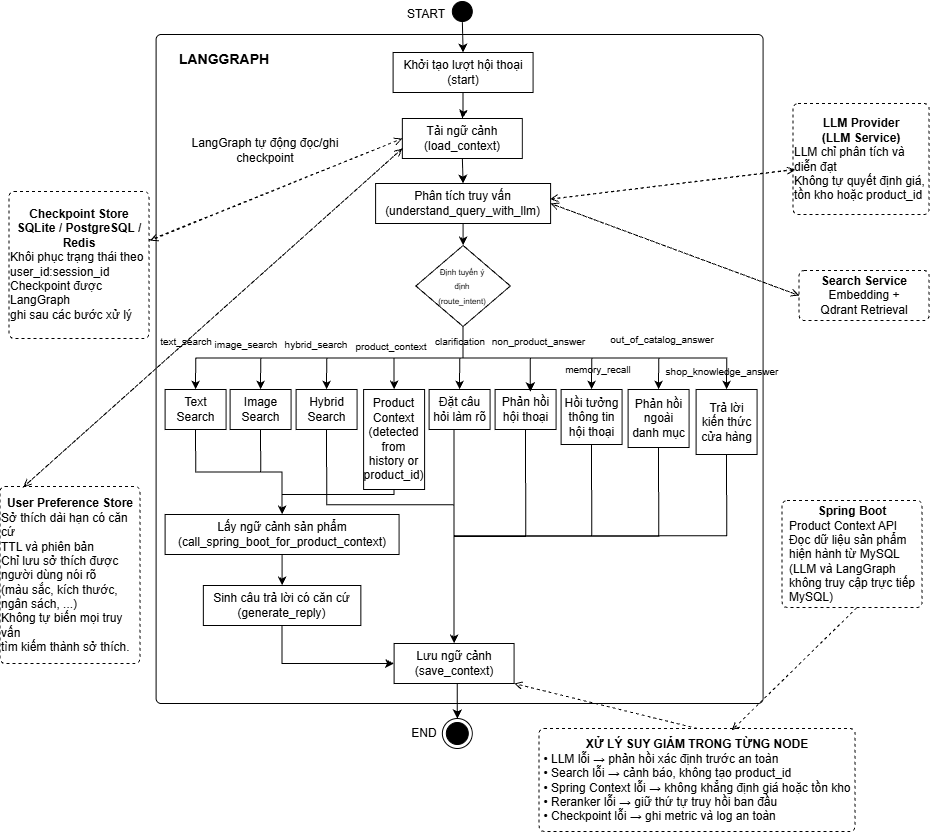
\includegraphics[width=0.96\textwidth,height=0.80\textheight,keepaspectratio]{Images/Thietkehethong/Thiết kế đồ thị trạng thái của trợ lý hội thoại.drawio.png}
    \caption{Thiết kế đồ thị trạng thái của trợ lý hội thoại}
    \label{fig:assistant-state-graph}
\end{figure}

Luồng tương tác giữa người dùng, Backend và AI Service đã được trình bày tại Hình~\ref{fig:activity-multiturn-chat}. Hình~\ref{fig:assistant-state-graph} mô tả workflow LangGraph: phiên nạp checkpoint, phân tích ý định, định tuyến đến tìm kiếm hoặc nhánh hội thoại, lấy ngữ cảnh sản phẩm rồi sinh câu trả lời và lưu trạng thái.

Các nhánh hỏi làm rõ, hội thoại thông thường và truy vấn ngoài danh mục đều kết thúc tại \texttt{save\_context}. Trợ lý không truy cập trực tiếp MySQL; khi LLM, Search Service hoặc checkpoint lỗi, hệ thống dùng kết quả còn có thể xác minh hoặc trả lời suy giảm, không tự tạo giá, tồn kho hay mã sản phẩm.

\subsection{Thiết kế giao tiếp, bảo mật và xử lý lỗi}

Frontend chỉ sử dụng API công khai của Spring Boot; dịch vụ nội bộ và lỗi phụ thuộc
được bảo vệ, chuẩn hóa để không ảnh hưởng đến nghiệp vụ thương mại điện tử.
Mỗi request đi qua Backend đều được kiểm tra danh tính, quyền truy cập và dữ liệu
đầu vào trước khi chuyển đến thành phần xử lý tương ứng. Cách tổ chức này giúp
Frontend không phải biết chi tiết triển khai của MySQL, Qdrant hay các mô hình AI.

\textbf{Hợp đồng giao tiếp giữa các dịch vụ.}

Frontend gọi API công khai của Spring Boot; Backend xác thực, kiểm tra quyền và gọi
AI Service qua API nội bộ. Hai dịch vụ trao đổi JSON bằng DTO tối giản, dùng
\texttt{product\_id} làm khóa liên kết; AI Service không nhận JPA Entity, không truy
cập MySQL và không trả payload nội bộ cho Frontend. API quản trị dùng tiền tố
\texttt{/admin}, API nội bộ dùng \texttt{/internal}; các thao tác đồng bộ hỗ trợ
chạy toàn bộ, tăng dần hoặc theo từng sản phẩm.

Indexing DTO chứa dữ liệu cần thiết để tạo embedding và payload Qdrant; search
response chỉ trả ứng viên, điểm, nguồn và cảnh báo; assistant response bổ sung câu
trả lời, mã phiên và các sản phẩm có căn cứ.
Các trường bắt buộc, giới hạn kích thước và định dạng dữ liệu được kiểm tra ở cả
hai phía của kết nối. Với thao tác đồng bộ, Backend có thể gửi lại cùng một sản
phẩm mà không tạo bản ghi trùng nhờ cơ chế upsert theo \texttt{product\_id} và
thời điểm cập nhật. Các hợp đồng chính được tổng hợp trong
Bảng~\ref{tab:spring-ai-contracts}.

\begin{breakabletable}
    \centering
    \caption{Các hợp đồng chính giữa Spring Boot và AI Service}
    \label{tab:spring-ai-contracts}
    \begin{tabularx}{\textwidth}{|p{0.18\textwidth}|p{0.36\textwidth}|X|}
        \hline
        \textbf{Hợp đồng} & \textbf{Dữ liệu chính} & \textbf{Ràng buộc thiết kế} \\
        \hline
        Index product & Product ID, text fields, attributes, price, stock, images, updated time & Upsert theo Product ID; không phụ thuộc cấu trúc JPA Entity. \\
        \hline
        Search & Modality, query/image, ROI, filters, top-k, candidate IDs, score & Giới hạn đầu vào; candidate phải được resolve lại và không thay thế giá/tồn kho. \\
        \hline
        Assistant & Session ID, message, context tối thiểu, answer, candidate IDs & Không truyền dữ liệu nhạy cảm không cần thiết; metadata nội bộ không trả ra giao diện. \\
        \hline
    \end{tabularx}
\end{breakabletable}

\textbf{Bảo mật tại các lớp giao tiếp.}

Request người dùng được xác thực bằng JWT; Backend tiếp tục kiểm tra vai trò và
quyền sở hữu tài nguyên. Kết nối nội bộ dùng \texttt{X-Internal-API-Key}, còn
MySQL, Qdrant và endpoint nội bộ chỉ được truy cập trong mạng được phép. Token,
mật khẩu, thông tin thanh toán và toàn bộ JPA Entity không được truyền sang AI;
secret đọc từ biến môi trường hoặc cơ chế quản lý bí mật.

Spring Boot và AI Service cùng kiểm tra schema, kích thước ảnh, ROI, top-k và
filter. Log chỉ ghi correlation ID và mã lỗi cần thiết, không ghi khóa hoặc nội
dung nhạy cảm. Quyền quản trị được kiểm tra riêng tại Backend; việc có thể gọi
được endpoint không đồng nghĩa với việc người dùng được phép truy cập mọi tài
nguyên. Các khóa tích hợp được cấu hình bên ngoài mã nguồn và có thể thay đổi
định kỳ khi cần.

\textbf{Chuẩn hóa lỗi, timeout và cơ chế suy giảm.}

Integration client cấu hình connection/read timeout và correlation ID. Lỗi đầu vào
trả về 4xx, lỗi xác thực/phân quyền trả về 401/403, lỗi phụ thuộc trả về 502/503
và lỗi không dự kiến trả về 500; Frontend chỉ dựa vào mã lỗi và trạng thái HTTP.

Retry chỉ áp dụng cho lỗi tạm thời và thao tác có tính lặp; indexing có thể gọi lại
nhờ \texttt{product\_id}, còn checkout không retry nếu chưa có idempotency key. Khi
AI lỗi, tìm kiếm văn bản dùng keyword fallback và các nghiệp vụ cốt lõi vẫn hoạt
động. Nếu không thể xác minh dữ liệu bắt buộc cho checkout, transaction phải dừng;
nếu chỉ reranker lỗi, kết quả truy hồi ban đầu vẫn được sử dụng. Frontend hiển thị
thông báo phù hợp theo nhóm lỗi, trong khi chi tiết kỹ thuật được giữ trong log để
phục vụ kiểm tra. Nhờ đó hệ thống vừa bảo đảm an toàn dữ liệu, vừa duy trì được
khả năng sử dụng khi một dịch vụ phụ trợ tạm thời không sẵn sàng.

\subsection*{Kết chương}

Chương này trình bày kiến trúc, dữ liệu, chức năng, giao tiếp, bảo mật và xử lý lỗi
của hệ thống. Spring Boot kiểm soát nghiệp vụ và là cổng giao tiếp duy nhất của
Frontend; MySQL là nguồn dữ liệu chuẩn, còn Qdrant và các thành phần AI là các
thành phần dẫn xuất có thể đồng bộ hoặc tái tạo độc lập. Thiết kế này bảo đảm các
chức năng cốt lõi như quản lý sản phẩm, giỏ hàng và đơn hàng vẫn được bảo vệ khi
dịch vụ AI hoặc một tích hợp bên ngoài gặp sự cố.
